%%%%%%%%%%%%%%%%%%%%%%%%%%%%%%%%%%%%%%%%%%%%%%%%%%%%%%%%%%%%%%%%%%%%%%%%%%%

\documentclass{standalone}

\usepackage{mathptmx}
\usepackage{tikz}
\usetikzlibrary{external}
\tikzexternalize{polar-cartesian}

%% We default to Times.
\renewcommand{\rmdefault}{ptm}
\renewcommand{\ttdefault}{pcr}
%% Enable Times/Palatino main text font.
\normalfont\selectfont

\newcommand{\comma}{,\,}
\newcommand{\tuple}[2]{(#1\comma #2)}

%% The Cartesian coordinate system.
\newcommand{\cartesianCoordinate}{%%
  %% The x-axis.
  \draw[axisStyle] (xstart) -- (xend);
  \node at (xend) [right] {$x$};
  %% The y-axis.
  \draw[axisStyle] (ystart) -- (yend);
  \node at (yend) [above] {$y$};
}

%% The radius.
\newcommand{\radiusLine}{%%
  %% A line as the radius
  \draw[dashStyle] (origin) -- (\xa,\yb);
  \node at (\xa/2,\yb/2+0.1) [above] {$r$};
  %% Label the angle.
  \draw[->,thick] (0.5,0) +(0:0.5cm) arc[start angle=0,radius=1,delta angle=45];
  \node at (0.9,0.4) [right] {$\varphi$};
}

%% A horizontal line.
\newcommand{\horizontalLine}{%%
  \node at (\xa/2,0) [below] {$r \cos \varphi$};
}

%% A vertical line meets at the generic point.
\newcommand{\verticalLine}{%%
  \draw[dashStyle] (\xa,0) -- (\xa,\yb);
  \node at (\xa,\yb/2) [right] {$r \sin \varphi$};
}

%% A point on the Cartesian plane.
%%
%% #1 -- The x-coordinate of the point.
%% #2 -- The y-coordinate of the point.
%% #3 -- Label the point with this name.
%% #4 -- Where to place the label relative to the point.
\newcommand{\xyPoint}[4]{%%
  \node[nodeStyle] at (#1,#2) {};
  \node at (#1,#2) [#4] {$#3$};
}

%% Converting from polar to Cartesian coordinates.

\begin{document}

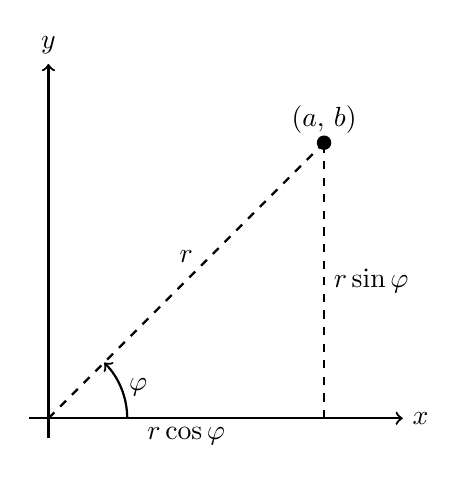
\begin{tikzpicture}[%%
  axisStyle/.style={->,thick},%%
  dashStyle/.style={-,thick,dashed},%%
  nodeStyle/.style={draw,inner sep=1.7pt,circle,fill=black,black}
]
%%
%%
\pgfmathsetmacro{\xa}{3.5}
\pgfmathsetmacro{\xhigh}{4.5}
\pgfmathsetmacro{\xlow}{-0.25}
\pgfmathsetmacro{\yb}{\xa}
\pgfmathsetmacro{\yhigh}{4.5}
\pgfmathsetmacro{\ylow}{-0.25}
\coordinate (origin) at (0,0);
\coordinate (xend) at (\xhigh,0);
\coordinate (xstart) at (\xlow,0);
\coordinate (yend) at (0,\yhigh);
\coordinate (ystart) at (0,\ylow);
%%
%%
%% Illustrate how to convert from polar to Cartesian coordinates.
\cartesianCoordinate
%% A generic point.
\xyPoint{\xa}{\yb}{\tuple{a}{b}}{above}
\radiusLine
\verticalLine
\horizontalLine
\end{tikzpicture}

\end{document}
